\documentclass[11pt]{article}
\usepackage{geometry}                % See geometry.pdf to learn the layout options. There are lots.
\geometry{a4paper}                   % ... or a4paper or a5paper or ... 
\usepackage{graphicx}
\usepackage{amssymb}
\usepackage{epstopdf}
\usepackage{tikz} % allows for figures
\usepackage{float} % allows [H] on figure definition
\usepackage{wrapfig}
\usepackage{amsmath} % allows for matrix 
\usepackage{amsthm} % definition environment
\usepackage[utf8]{inputenc}
\usepackage[english]{babel}
\usepackage{subfig}

\DeclareGraphicsRule{.tif}{png}{.png}{`convert #1 `dirname #1`/`basename #1 .tif`.png}

\graphicspath{ {images/} }

% user macros
% comamnds
\newcommand{\R}{\mathbb{R}}
\newcommand{\C}{\mathbb{C}}
\newcommand{\CP}{\hat{\mathbb{C}}}

% environments
\newtheorem{theorem}{Theorem}[section]
\newtheorem{corollary}{Corollary}[theorem]
\newtheorem{lemma}[theorem]{Lemma}
\theoremstyle{definition}
\newtheorem{definition}{Definition}[section]

% end user macros

\title{Equivalent Representations of Circle Packings}
\author{
  Kevin Pratt\\
  \texttt{kevin.pratt@uconn.edu}
  \and
  Connor Riley\\
  \texttt{connor.t.riley@gmail.com}
    \and
  Donald R. Sheehy\\
  \texttt{don.r.sheehy@uconn.edu}
}\date{April 2016}

\begin{document}

\maketitle

\begin{abstract}
  We explore equivalent representations of circle packings and the relationships between them connecting them to theorems by Maxwell and Tutte.  
  The associated code is available at a website as noted and cited in the introduction.
\end{abstract}

\section{Introduction}

\begin{wrapfigure}{r}{0.4\textwidth}
  \begin{center}
    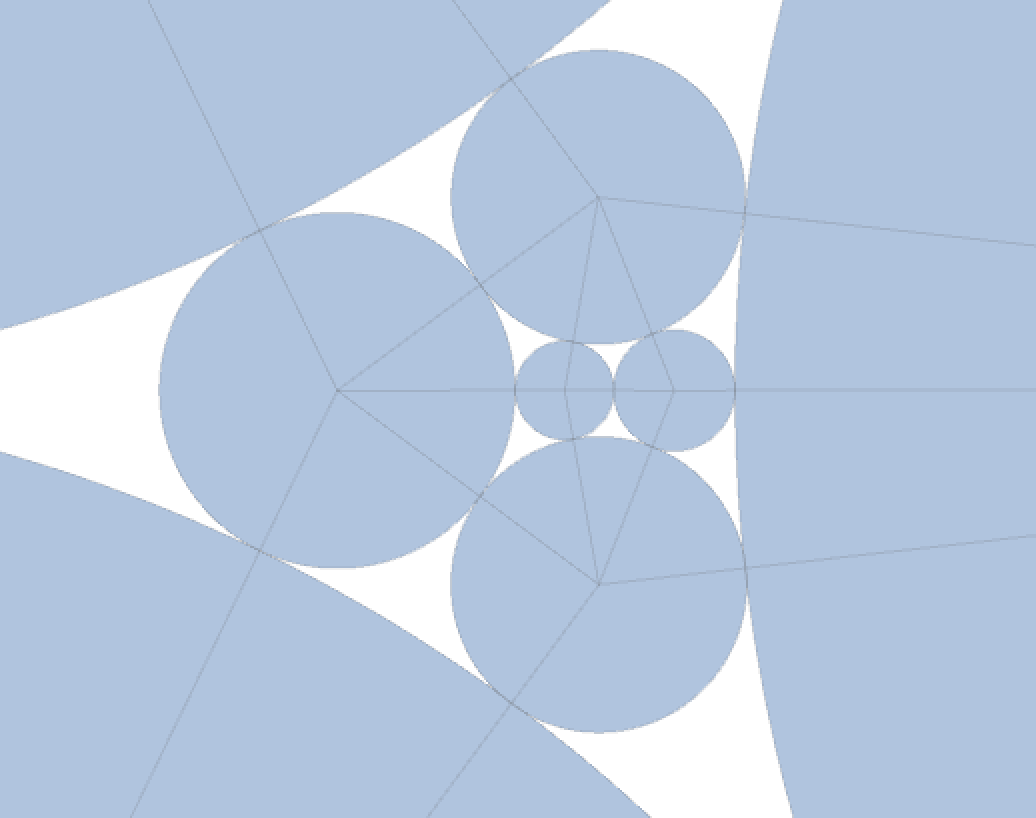
\includegraphics[scale=.18,width=0.45\textwidth]{circlepacking_1}
  \end{center}
  \caption{A univalent circle packing in a triangle.}
\end{wrapfigure}

	The Circle Packing Theorem provides a link between questions of geometry, topology, combinatorics and complex analysis. 
	Discovered by Paul Koebe and later reintroduced by William Thurston, circle packings have become a principle area of study for many mathematicians and geometers \cite{wilkerson}. 
	Before introducing a formal definition, we will develop an intuition for circle packings. 
	A circle packing is a configuration of circles with a specified pattern of tangencies \cite{stephenson05introduction}. 
	The circle packings most often studied are those that require the interior of the circles to be disjoint, called univalent packings, this means the circles are non-overlapping \cite{stephenson05introduction}. 
	In this case, a circle packing can be thought of as a graph formed by a set of circles with disjoint interiors, where each circle kisses, intersects at exactly one point, its neighboring circles in the graph.

	Common geometric settings for circle packings are the \emph{Euclidean plane}, the \emph{sphere} and the \emph{hyperbolic plane}. 
	Each pair of circles in a packing forms a \emph{tangent pair}, every three form a \emph{triple} and the empty space between each triple forms an $interstice$ \cite{stephenson05introduction}. 
	A $flower$ is the next level of structure, which consists of a central circle and some number of $petal$ circles. 
	The number of petals defines the $degree$ of the central circle. 
	In the visualization tool used to create the circle packing figures we enforce the condition that every circle packing has to have a flower. 
	Note that while not all circle packings are univalent, the ones discussed in this paper and created by the visualization tool will all be univalent \cite{visualizationTool}. 
	As a result of this property the angle sum, the sum of the angles around each vertex, will be $2\pi$.

	The primary objective of this paper is to explore the connections between equivalent representations of circle packings. 
	These representations include Delaunay triangulations, liftings, stresses, and packings on the sphere. 
	The secondary goal is to introduce the reader to the world of circle packings. To this end, basic Geometric principles will be introduced.

\section{Introduction to Geometric Figures}
\subsection{Graphs}
	\theoremstyle{definition}
	\begin{definition}{\textsc{Graph}}
		A \emph{graph} is an ordered pair $G=(V,E)$ which represents a set of objects or \emph{vertices} $v$ and the links between them, or \emph{edges} $E$. 
		Edges in a graph can be directed or undirected, however, we will focus on undirected edges in our application. 
	\end{definition}
	
	\theoremstyle{definition}
	\begin{definition}{\textsc{Directed Graph}}
  		A \emph{directed graph} is a graph in which each edge is an ordered pair of vertices.
	\end{definition}
	
	\theoremstyle{definition}
	\begin{definition}{\textsc{Undirected Graph}}
  		A \emph{undirected graph} is a graph in which each edge is an unordered pair of vertices such that $(v_1, v_2) = (v_2, v_1)$.
  	\end{definition}
	
	\theoremstyle{definition}
	\begin{definition}{\textsc{Subgraph}}
			If graph $G$ is undirected then, a graph $G' = (V',E')$ is a \emph{subgraph} of $G$ ($G' \subseteq G$), if $V' \subseteq V$ and $E' \subseteq E$.
  	\end{definition}

	\theoremstyle{definition}
	\begin{definition}{\textsc{Path}}
		A \emph{path} is a finite or infinite sequence of edges which connect a sequence of vertices.
	\end{definition}
	
	\theoremstyle{definition}
  	\begin{definition}{\textsc{Connected Component}}
		A component or \emph{connected component} of a graph is a subgraph in which any two vertices are connected to each other by a path which is connected to no additional vertices in the supergraph.
	\end{definition}
	
	\theoremstyle{definition}
	\begin{definition}{\textsc{Self-Loop}}
  		A \emph{self-loop} is an edge connecting a vertex to itself.
  	\end{definition}
	
	\theoremstyle{definition}
	\begin{definition}{\textsc{Multiple Edges}}
  		A graph with \emph{multiple edges} is one which has two or more edges connect the same two vertices.
	\end{definition}
	
	\theoremstyle{definition}
	\begin{definition}{\textsc{Connected Graph}}
		A graph is \emph{connected} when there is a path between every pair of vertices \cite{mathworld:ConnectedGraphs}. 
	\end{definition}

	In a connected graph every vertex is reachable. A graph with just one vertex is connected. 
	A graph is said to be \emph{k-vertex-connected} if there does not exist a set of k-1 vertices whose removal disconnects the graph. 
	Additionally, a graph is \emph{k-edge-connected} if there does not exist a set of k-1 edges whose removal disconnects the graph. 
	Typically we will work with 3-vertex-connected graphs, which will be referred to as 3-connected for short.

	\theoremstyle{definition}
	\begin{definition}{\textsc{Simple Graph}}  
  		A \emph{simple graph} is an unweighted, undirected graph, containing no loops or multiple edges \cite{mathworld:SimpleGraphs}. 
	\end{definition}
	
	A simple graph may either be connected or disconnected.
	
	\theoremstyle{definition}
	\begin{definition}{\textsc{Contraction}}
		The contraction of a pair of vertices $v_1$ and $v_2$ of a graph produces a graph in which the two vertices are replaced with a single vertex $v$ such that $v$ is adjacent to the union of the vertices to which $v_1$ and $v_2$ were originally adjacent. 
		If the vertices $v_1$ and $v_2$ are connected by an edge then the edge is removed \cite{mathworld:Contraction}.
	\end{definition}
	
\subsubsection{Embeddings and Topology}
    
    \begin{wrapfigure}{r}{.4\textwidth}%
		\centering
		\subfloat[An embedding of a graph in the plane.]{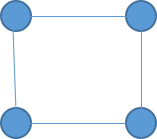
\includegraphics[width=.15\textwidth]{embedding1}}%
		\qquad
		\subfloat[A different embedding of the same graph in the plane.]{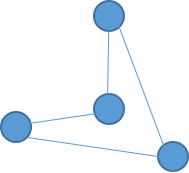
\includegraphics[width=.15\textwidth]{embedding2}}%
		\caption[]{Embeddings of the graph in the plane.}%
		\label{fig:embedding}
	\end{wrapfigure}
    
    	An \emph{embedding} of a graph $G$ on a surface $\Sigma$ is a representation of $G$ on $\Sigma$ in which points of $\Sigma$ are associated to vertices and simple arcs are associated to edges in such a way that:
  		\begin{itemize}
			\item The endpoints of the arc associated to the edge $e$ are the points associated to the end vertices of $e$.
			\item No arcs include points associated with other vertices.
			\item Two arcs never intersect at a point which is interior to either of the arcs.
  		\end{itemize}

	This can be stated mathematically as the following: 
	\theoremstyle{definition}
	\begin{definition}{\textsc{Embedding}}
		Given edges $e=(u,v)$, the function mapping the vertices to the plane $ \phi :V \rightarrow \R^2$, and the function mapping the edges to the plane $ \rho_e :[0,1] \rightarrow \R^2$, the embedding $= \langle \phi, \{\rho_e : e \in E \} \rangle$. 
	\end{definition}
		The difference between a graph and an embedding can best be illustrated with an example. 
		Essentially, a graph $G=(V,E)$ just defines the structure, whereas an embedding defines the positioning of the graph in the plane.
	
	\theoremstyle{definition}
	\begin{definition}{\textsc{Straight-Line Embedding}}
		A \emph{straight-line embedding} is a embedding of a planar graph in which all arcs are straight. The figures from the example above are straight-line embeddings.
  	\end{definition}
	
	\theoremstyle{definition}
	\begin{definition}{\textsc{Planar Graph}}
		A \emph{planar graph} is one that can be embedded in the plane.
	\end{definition}
	
	In other words, the graph can be drawn on the plane in such a way that its edges intersect only at their endpoints (no edges cross each other) \cite{mathworld:PlanarGraph}.
	
	\theoremstyle{definition}
	\begin{definition}{\textsc{Face}}
		A face of a planar straight-line graph is a set of edges ${e_1,...e_k}$ which bounds an area of the plane such that it contains no edges.
		In other words, the faces are the boundaries of the connected components of $\R^2 \setminus \pi(G)$.
	\end{definition}
	
	\theoremstyle{definition}
	\begin{definition}{\textsc{Planar Straight-Line Graph}}
		A planar straight line graph is a graph that can be embedded in the plane where all the edges are straight lines. $PSLG = (V,E,F, \{\pi : V \rightarrow \R^2 \})$, where a face of a PSLG is a set of edges.
	\end{definition}
	
	\theoremstyle{definition}
	\begin{definition}{\textsc{Dual Graph}}
		The \emph{dual graph} $G'$ of a planar graph $G$ is one whose vertices each corresponds to a face in $G$. 
		Two vertices are connected by an edge if the corresponding faces in $G$ have a boundary edge in common \cite{mathworld:dualGraph}. 
  	\end{definition}
	%\theoremstyle{definition}
	%\begin{definition}{\textsc{Simplex}}
	%	A \emph{simplex} is the generalization of a triangle to arbitrary dimensions.
	%\end{definition}

\subsubsection{Matrix Manipulation and Terminology}

	\theoremstyle{definition}
	\begin{definition}{\textsc{Eigenvalues}}
		Let $A$ be a linear transformation represented by a matrix. If there is a vector $X \in \R^n \neq 0$ such that $AX = \lambda X$ for some scalar $\lambda$, then $\lambda$ is called the \emph{eigenvalue} of $A$ \cite{mathworld:Eigenvalue}.
	\end{definition}
	
	\theoremstyle{definition}
	\begin{definition}{\textsc{Diagonal Matrix}}
		A \emph{diagonal matrix} is a square matrix of the form \cite{mathworld:DiagonalMatrix}:
		$\begin{bmatrix}
			c_1 & 0 & \dots & 0 \\
			0 & c_2 & \dots & 0 \\
			\vdots & \vdots  & \ddots  & \vdots \\
			0 & 0 & \dots & c_n \\
		\end{bmatrix}$. These matrices are sometimes written $D = \text{diag}(c_1, \dots, c_n)$
	\end{definition}
	
	\theoremstyle{definition}
	\begin{definition}{\textsc{Identity Matrix}}
		The \emph{identity matrix} is the diagonal matrix $I = \text{diag}(1, \dots, 1)$.
	\end{definition}
	
	\theoremstyle{definition}
	\begin{definition}{\textsc{Adjacency Matrix}}
		An \emph{adjacency matrix}, $A$, of a simple labeled graph is a matrix with rows and columns labeled by graph vertices, with a 1 or 0 in position (i, j) according to whether $v_i$ and $v_j$ are adjacent (joined by an edge) or not \cite{mathworld:AdjacencyMatrix}. 
	\end{definition}
	
	\theoremstyle{definition}
	\begin{definition}{\textsc{Characteristic Polynomial}}
		The \emph{characteristic polynomial} is the polynomial left-hand side of the characteristic equation: $\det(A - \lambda I) = 0$ \cite{mathworld:CharacteristicPoly}.
	\end{definition}
	
	\theoremstyle{definition}
	\begin{definition}{\textsc{Transpose}}
		A \emph{transpose} of a matrix $M$, written $M^T$, is the matrix obtained by replacing all elements $m_{ij}$ with $m_{ji}$ \cite{mathworld:Transpose}.
	\end{definition}
	
	\theoremstyle{definition}
	\begin{definition}{\textsc{Symmetric Matrix}}
		A \emph{symmetric matrix} is a square matrix that satisfies $A^T = A$ \cite{mathworld:SymmetricMatrix}.
	\end{definition}
	
	\theoremstyle{definition}
	\begin{definition}{\textsc{Vertex Degree}}
		The \emph{vertex degree} of a vertex is the number of edges attached to that vertex \cite{mathworld:VertexDegree}.
	\end{definition}
	
	\theoremstyle{definition}
	\begin{definition}{\textsc{Out Degree}}
		The number of outward directed graph edges from a given vertex in a directed graph.
	\end{definition}
	
	\theoremstyle{definition}
	\begin{definition}{\textsc{Degree Matrix}}
		A \emph{degree matrix} is a diagonal matrix where the diagonal $d_i$ corresponds to the vertex degree of $v_i$ \cite{mathworld:DegreeMatrix}. 
	\end{definition}
	
	\theoremstyle{definition}
	\begin{definition}{\textsc{Laplacian}}
		A \emph{Laplacian} of a graph $G$ is an $n \times n$ symmetric matrix with one row and one column for each vertex defined by $L = D - A$, where $D$ is the degree matrix and A is the adjacency matrix \cite{mathworld:Laplacian}.
	\end{definition}

\subsubsection{Misc.}
	\theoremstyle{definition}
	\begin{definition}{\textsc{Bijection}}
		A map is called \emph{bijective} it is both a one-to-one and an onto map. 
		Essentially, it is one-to-one and invertible. \cite{mathworld:Bijection}. 
	\end{definition}
	
	\theoremstyle{definition}
	\begin{definition}{\textsc{Permutation}}
		 A \emph{permutation} is a rearrangement of the elements of an ordered list $S$ into a one-to-one correspondence with itself \cite{mathworld:Permutation}.
	\end{definition}
	
	\theoremstyle{definition}
	\begin{definition}{\textsc{Centroid}}
		A \emph{centroid} is the center of mass of a two-dimensional closed surface or three-dimensional solid \cite{mathworld:Centroid}.
	\end{definition}
	Now that we have defined general geometric, topological and matrix concepts, we may introduce the formal definition of a circle packing.

\section{Circle Packings}
	\theoremstyle{definition}
	\begin{definition}{\textsc{Circle Packing}}
		A collection $P = \{c_v\}$ of circles is said to be a circle packing for a graph $G$ if 
		(1) $P$ has a circle $c_v$ for each vertex $v$ of $G$, 
		(2) two circles $c_u$, $c_v$ are tangent whenever $(u,v)$ is an edge of $G$, and 
		(3) three circles $c_u$, $c_v$, $c_w$ form a triple whenever $(u,v,w)$ forms a face in $G$ \cite{stephenson05introduction}.
	\end{definition}

	By \textbf{Koebe's theorem}, circle packings exists for any maximal planar graph, however it is often simpler algorithmically to work with 3-connected, triangulated planar graphs.

	The first algorithm in our circle packing application is an incremental relaxation algorithm proposed by Stephenson in his book \emph{Introduction to Circle Packing}. 
	The algorithm begins with a set of tentative radii not necessarily corresponding to a valid packing. In our application, these radii are those input by the user. 
	The algorithm then performs the following steps:
	
	\begin{enumerate}
		\item Choose an internal vertex $v$ of the input graph.
		\item Calculate the total angle $\theta$ that its $k$ neighboring circles would cover around the circle for $v$, if the neighbors were placed tangent to each other and to the central circle using their tentative radii.
		\item Determine the radius $r$ for the neighboring circles, such that $k$ circles of radius $r$ would give the same covering angle $\theta$ as the neighbors of $v$ give.
		\item Set the new radius for $v$ to be the value for which $k$ circle of radius $r$ would give a covering angle of exactly $2\pi$.
	\end{enumerate}
	
	These steps cause the system to converge to a fixed point for which the sum of the angles around each vertex is $2\pi$. 
	Once the system has converged, the circles may be placed one at a time, at each step using the positions and radii of two neighboring circles to determine the center of each successive circle.

	\begin{figure}[H]%
    		\centering
    		\subfloat[User input]{{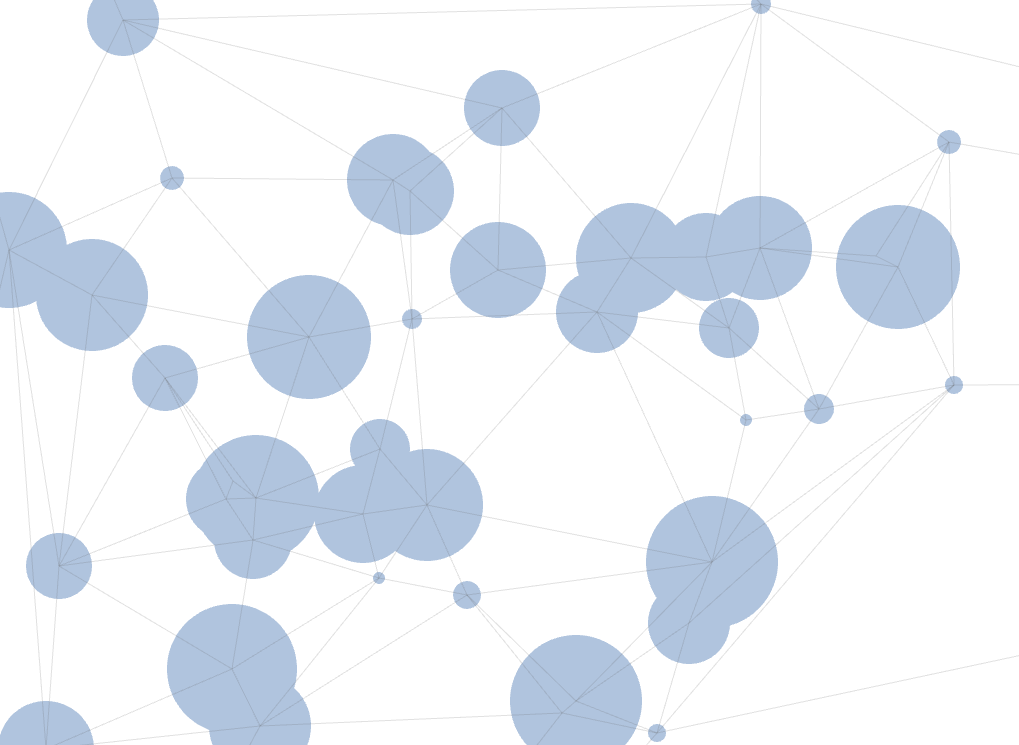
\includegraphics[width=.4\textwidth]{figures/input} }}%
    		\qquad
    		\subfloat[User input packed]{{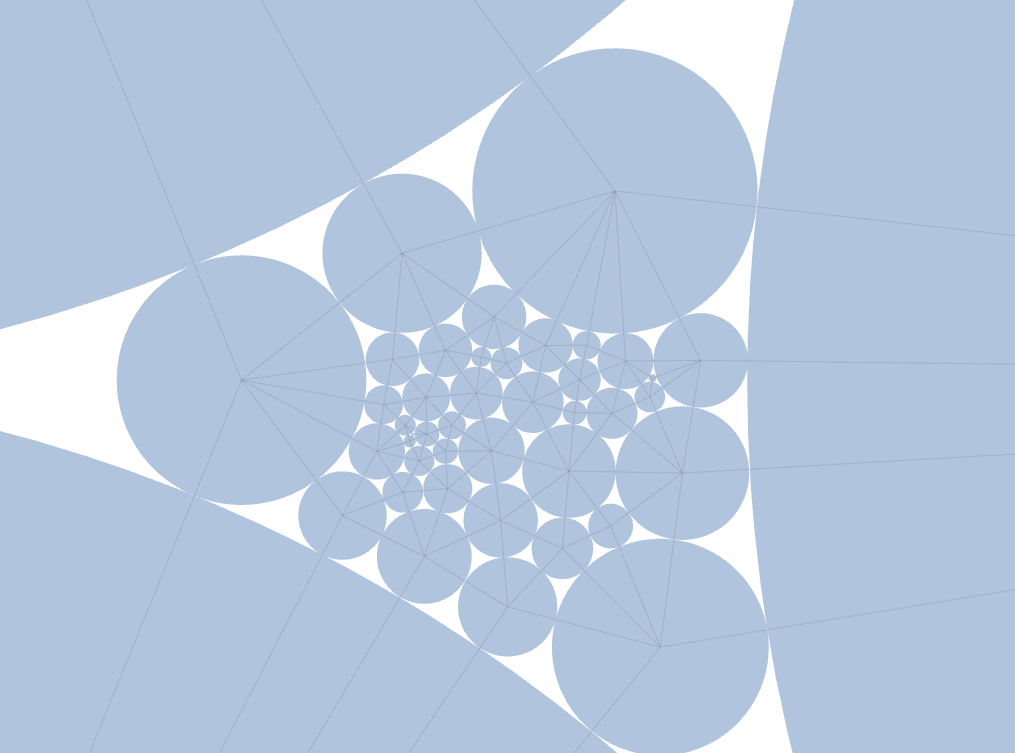
\includegraphics[width=.4\textwidth]{figures/output} }}%
    		\caption{Computing a circle packing}%
    		\label{fig:inout}%
	\end{figure}

\subsection{Delaunay Triangulations}
	
	\theoremstyle{definition}
	\begin{definition}{\textsc{Triangulation}}
		A \emph{triangulation}, straight-line planar graph in which every face is a triangle \cite{meshGeneration}. 
	\end{definition}

	There are many specific types of triangulations in mathematics, however, we will focus on Delaunay and Weighted Delaunay triangulations which are intimately connected to circle packings.
	To explain Delaunay triangulations, some properties of triangles must first be defined. 
	The \emph{circumcircle} of a triangle is the unique circle passing through its three vertices \cite{mathworld:Circumcenter}. 
	The center of the circumcircle is called the \emph{circumcenter} and the radius is the \emph{circumradius}. 
	The circumcenter can be found by finding the intersection of the three \emph{perpendicular bisectors} of the triangle which can be found by extending lines from the midpoint of each edge perpendicular to that edge.

  	\theoremstyle{definition}
  	\begin{definition}{\textsc{Delaunay Triangulation}}
		A \emph{Delaunay triangulation} for a set of points $P$ is the triangulation of those points such that no point in $P$ is inside the circumcircle of any other triangle \cite{meshGeneration}.
	\end{definition}
	
	The vertices in a Delaunay triangulation are the centers of the circles in a packing while the edges indicate tangencies between the circles.
	 In our visualization tool we show the Delaunay triangulation of the user's input. 
	 This triangulation is computed using the edge flip algorithm.	
	 
\subsubsection{The Edge Flip Algorithm}
	An edge $e$ in the triangulation $\tau$ is \emph{locally Delaunay}, if $e$ is an edge of fewer than two triangles, or if $e$ is an edge of exactly two triangles and it has an open circumcircle containing no vertex of either triangle. 
	A triangulation is Delaunay if it is locally Delaunay for every edge \cite{meshGeneration}.

	The union of any two triangles is a quadrilateral, and the shared edge is the diagonal of that quadrilateral. 
	To perform an edge flip is to replace the diagonal with the quadrilateral's other diagonal.

	\begin{wrapfigure}{r}{0.4\textwidth}
  		\begin{center}
    		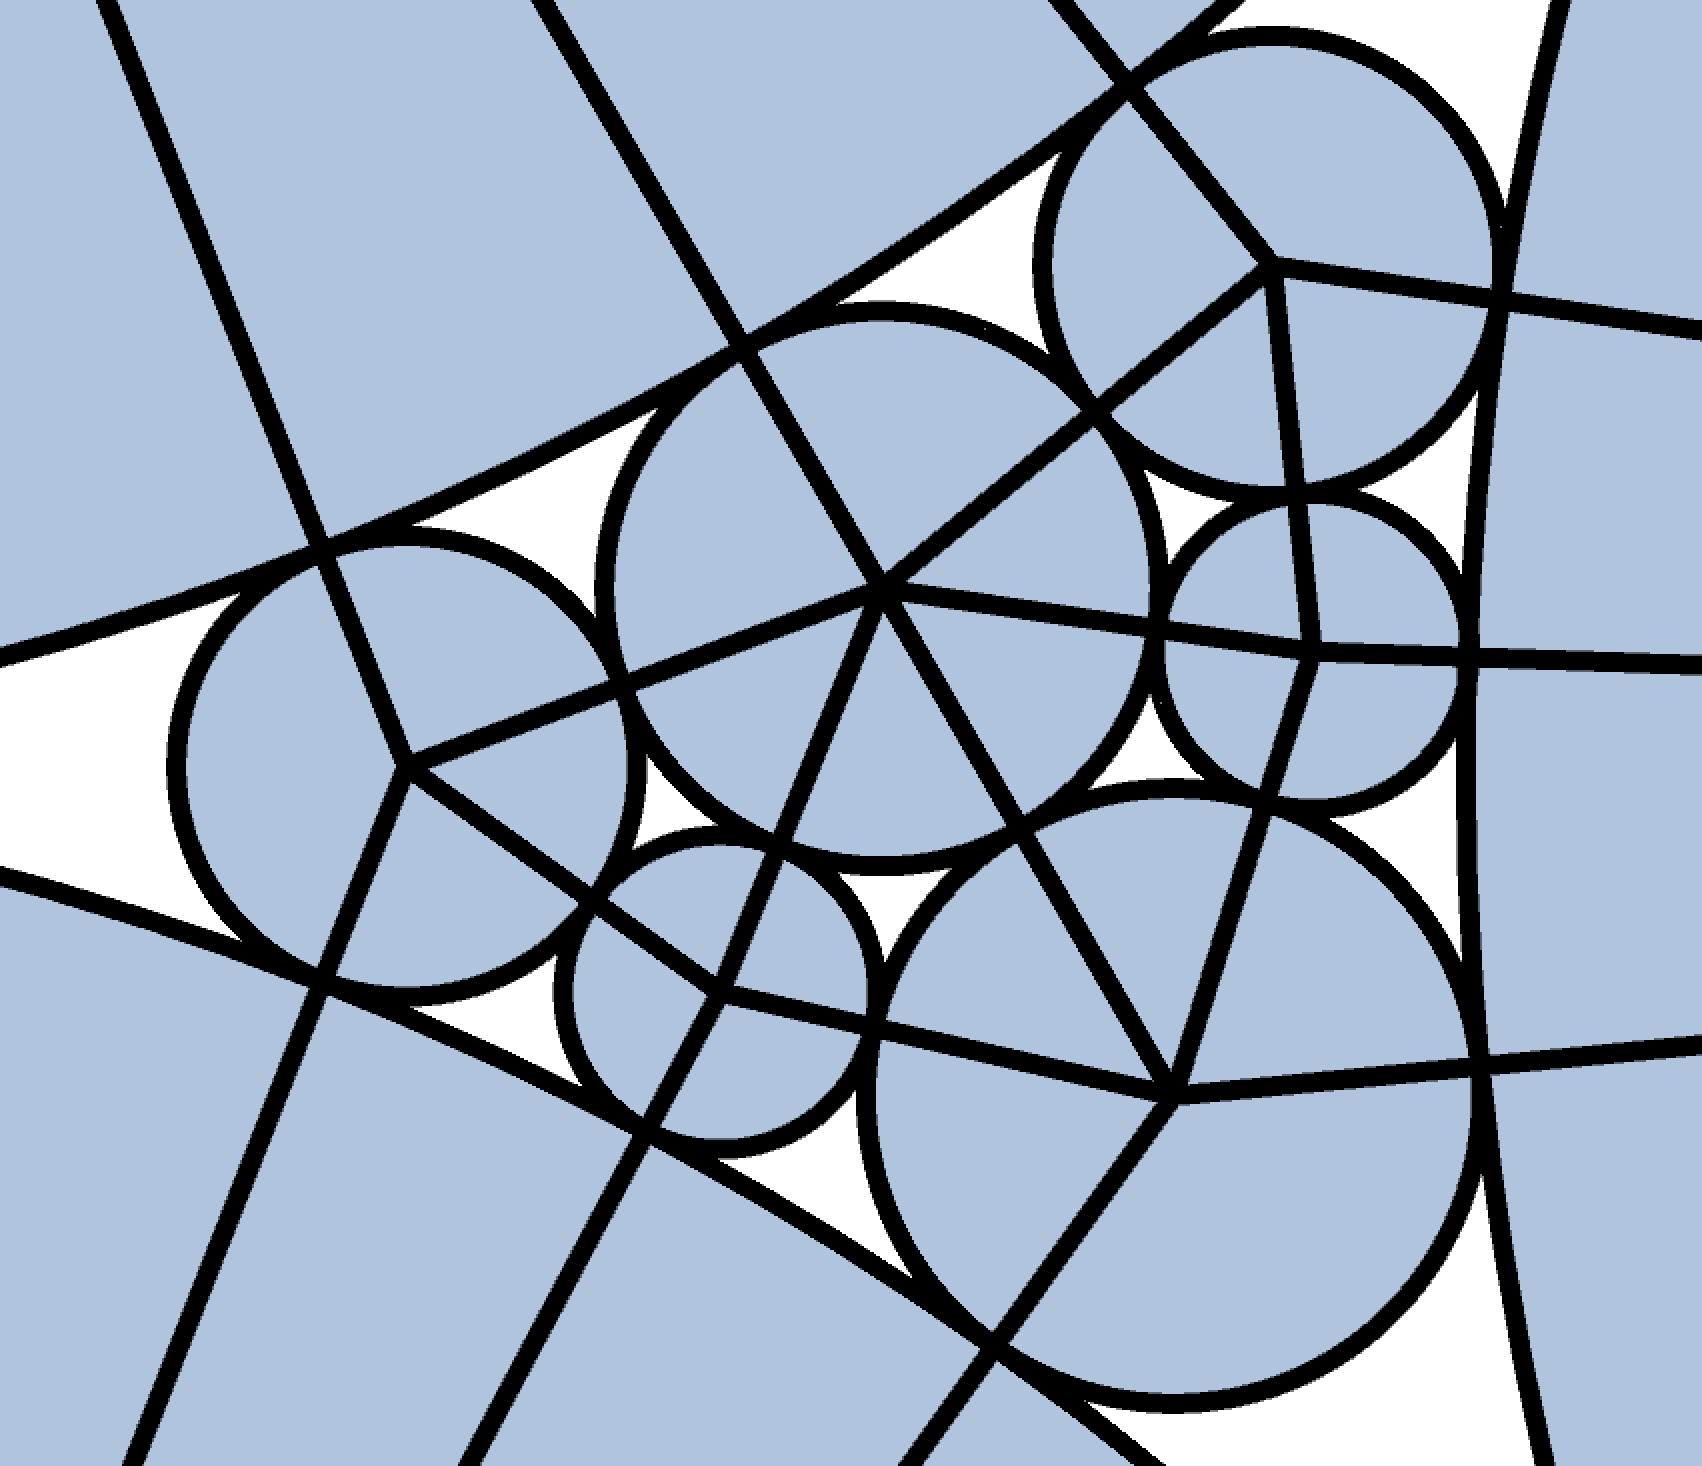
\includegraphics[width=0.38\textwidth]{delaunayemph}
  		\end{center}
  		\caption{Delaunay Triangulation in black.}
	\end{wrapfigure}
	As a result of this property, we can formulate an algorithm (the edge flip algoirthm) that creates a Delaunay triangulation. 
	If $S$ is the point set, this algorithm begins with any triangulation $\tau$ of $S$ and a list of edges in $\tau$. 
	Remove an edge from the list, check if the edge is still in the triangulation and if so, if it is locally Delaunay. 
	If the edge is present but not locally Delaunay, perform an edge flip and add the four surrounding edges to the list of edges to check. 
	This yields an $O(n + k)$ runtime, where $k$ is the number of flips performed and in the worst case $k = O(n^2)$ \cite{meshGeneration}.

	This leaves one issue, how do we determine whether an edge is locally Delaunay. 
	This can be done using the \emph{InCircle test}. 
	Given triangle $abc$ and point $p \in P$ $InCircle(a,b,c,d) \neq 1$ if $abc$ if Delaunay \cite{princeton:CCW}. 
	\begin{equation}
		InCircle(a,b,c,d) = \frac{sign(\det
		\begin{bmatrix}
    			a & b & c & d \\
    			\|a\|^2 & \|b\|^2 & \|c\|^2 & \|d\|^2 \\
    			1 & 1 & 1 & 1 \\
		\end{bmatrix} 
		)}{ccw(a,c,b)}
	\end{equation}
	\begin{equation}
		ccw(a,c,b) = \det[c-a,b-a] = \det
		\begin{bmatrix}
    			a & b & c \\
    			1 & 1 & 1\\
		\end{bmatrix} 
	\end{equation} 
	
	The \emph{counter clockwise test} or $ccw$ determines whither point $d$ is above or below the plane defined by points $a,b,c$. 
	This is because for any point $a = (x,y)$ the parabolic lifting is defined as $h(x,y) = x^2 + y^2 = \| 
	\begin{bmatrix} 
		x \\
		y \\ 
	\end{bmatrix} 
	\|^2$.
	As a result for any point $a$ the parabolic lifting of $a$, $a'$ is equal to $
	\begin{bmatrix} 
		a \\ 
		\| a \|^2 \\ 
	\end{bmatrix}$. 
	Therefore the lifting of all three points is equal to
	$\begin{bmatrix}
    			a & b & c \\
    			\|a\|^2 & \|b\|^2 & \|c\|^2 \\
	\end{bmatrix}$ 
	is the parabolic lifting of the points $a,b,c$.

	We can develop an incremental algorithm for finding Delaunay triangulations using, in part, the edge flip algorithm.
	Given a Delaunay triangulation and a point $p$ to add to the set of points $P$, a new Delaunay triangulation can be created containing point $p$ by first finding the triangle containing point $p$ and then splitting the triangle three ways. 
	This is done by creating edges from point $p$ to each vertex of the triangle. 
	Now that a we have a triangulation the edge flip algorithm is run to make it a Delaunay triangulation. 
	The base case of this algorithm is there are only three points, in which case, the points are connected to create a triangle \cite{meshGeneration}. 

\subsubsection{Voronoi Diagrams}

	\begin{wrapfigure}{r}{0.4\textwidth}
  		\begin{center}
    		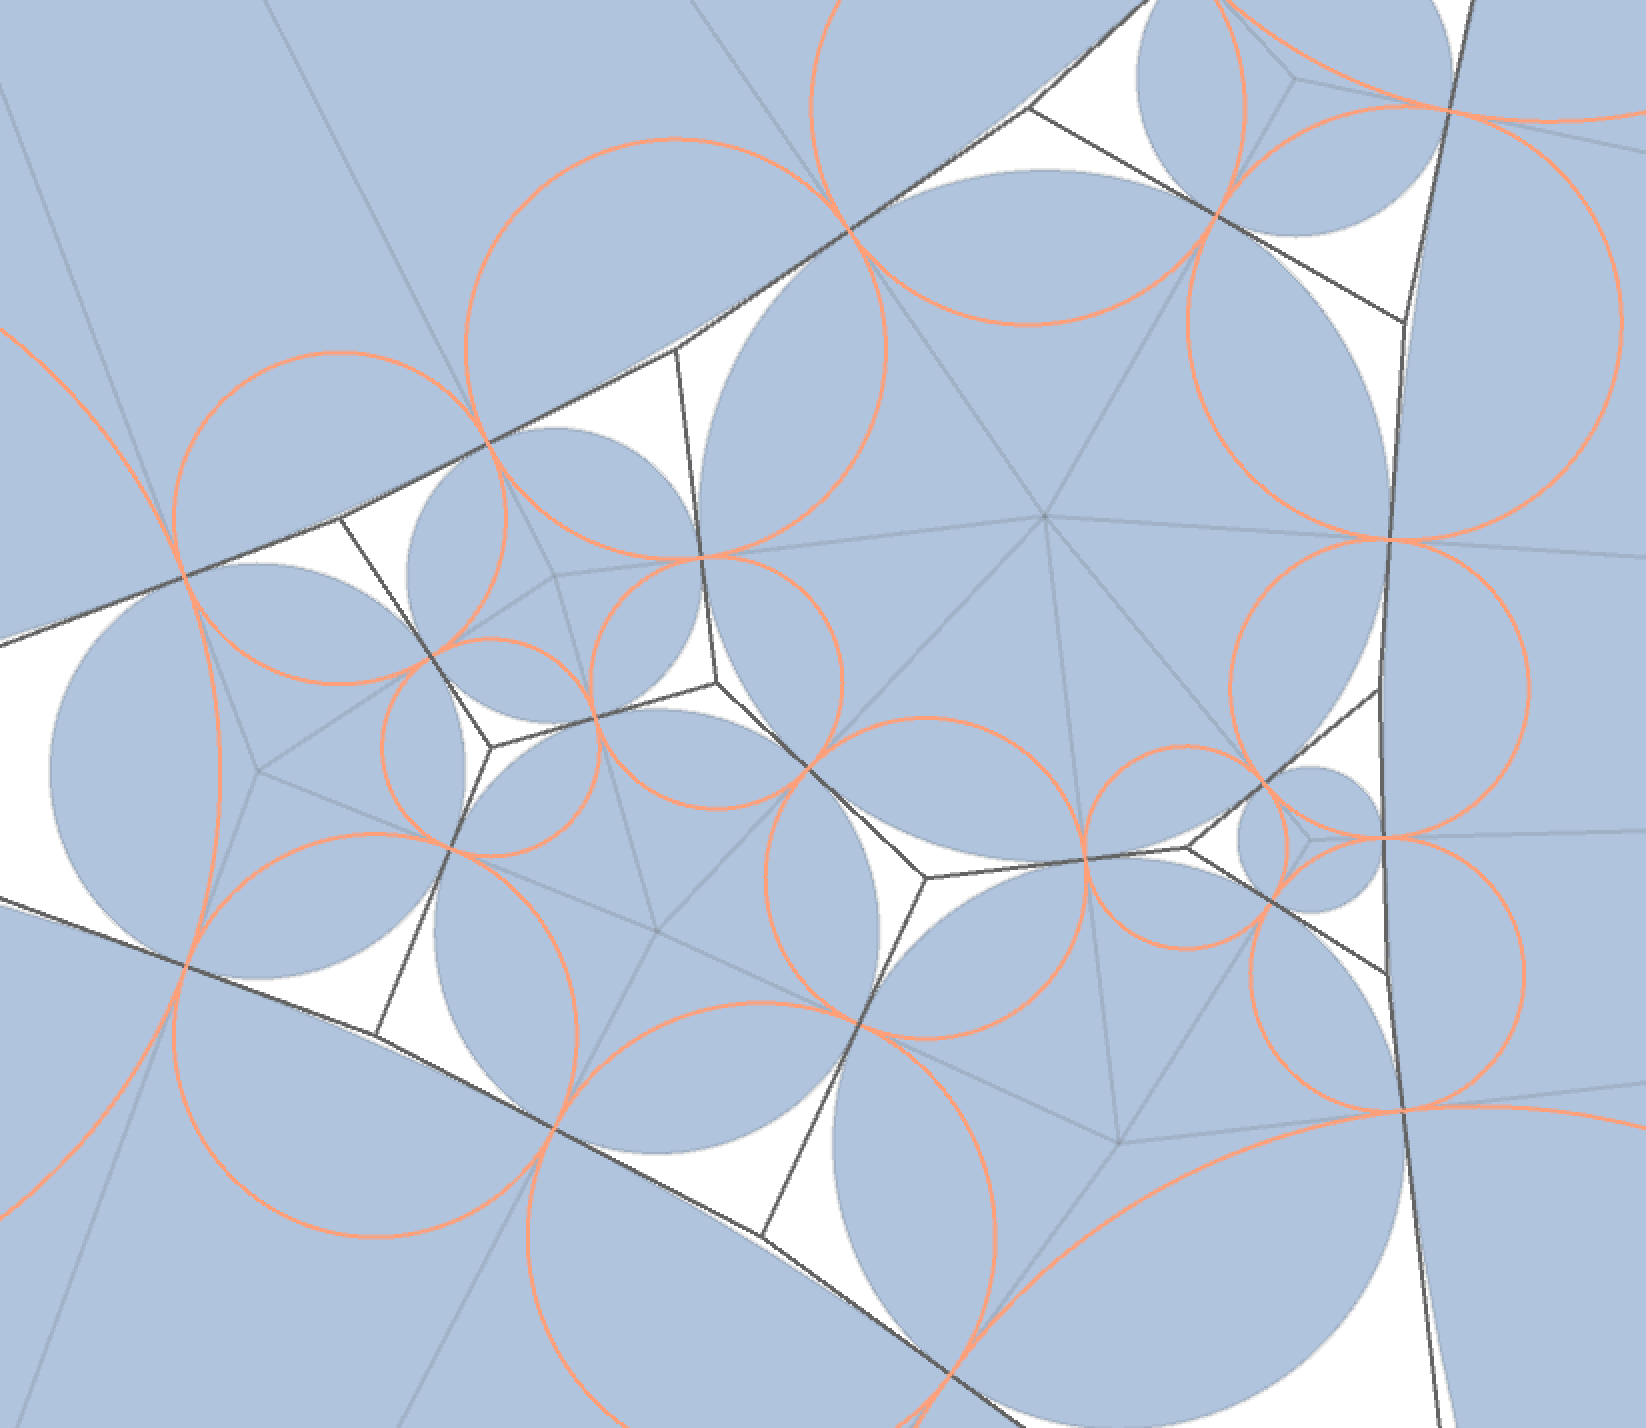
\includegraphics[scale=.18,width=0.45\textwidth]{voronoi}
  		\end{center}
  		\caption{A circle packing with its dual in red and the Voronoi diagram in black.}
	\end{wrapfigure}

	Voronoi diagrams are the geometric $dual$ of Delaunay triangulations. 
	A \emph{Voronoi diagram} is the partitioning of a plane into regions based on distance to points in a specific subset of the plane. 
	Formally, in Euclidean space each Voronoi cell $C_k$ is a convex polygon associated with a generator point $p_k$ where all locations in $C_k$ are closer to $p_k$ then any other generator point \cite{voronoiDiagrams}. 

	As a result of the dual relationship the faces, or 2-cells, of the Voronoi diagram correspond to the points of the Delaunay triangulation. 
	The edges, or 1-cells, of the Voronoi diagram correspond to the edges of the Delaunay triangulation and the vertices, or 0-cells, of the Voronoi diagram correspond to faces of the Delaunay triangulation.
	Lastly, the edges of the Voronoi Diagram are orthogonal to the edges of the Delaunay triangulation. 

	Each vertex of every cell in the Voronoi diagram is the center of a circle in the dual packing. 
	Additionally, if there is an edge of the from one vertex to another, the circles encompassing those vertices must kiss. 
	
	Interestingly, if you take the edge in the Delaunay triangulation that is orthogonal to a corresponding edge in the Voronoi diagram, the length from the vertex to the Voronoi edge is the length of the radius of the circle centered at that vertex.

\subsubsection{Weighted Delaunay Triangulations}
	The weighted Delaunay triangulation is the dual to the so-called power diagram, a Voronoi diagram on the points where the (squared) distance to a circle $c$ with center $p$ and radius $r$ is defined to be $\pi_c(x)^2 := \|x-p\|^2 - r^2$.
  	A circle packing representation of a graph realizes the graph as the weighted Delaunay triangulation where the vertices are the centers of the disks, the edges are the tangencies, and the weights are the radii.
  
\section{Embeddings, Liftings and Stress}
	
	From Koebe's theorem we know that every planar graph has a circle packing, however we will deal with 3-connected, triangulated graphs. 
	These graphs in particular allow us to easily examine other equivalent representations of circle packings. 
	In this section, we will explore the relationship between embeddings, liftings, stresses, and circle packings.

	First, we restate the mathematical definition of an embedding from above. 
	Given edges $e=(u,v)$, the function mapping the vertices to the plane $ \phi :V \rightarrow \R^2$, and the function mapping the edges to the plane $ \rho_e :[0,1] \rightarrow \R^2$, the embedding $= \langle \phi, \{\rho_e\} \in E \rangle$ \cite{mathworld:Embedding}.
	Second, a \emph{stress} is an assignment of values to edges that may be interpreted as spring constants. 
	By Hook's Law, the magnitude of the force exerted by a spring is the spring constant times its length. 
	A stress is an \emph{equilibrium stress} if for each vertex, the sum of the forces exerted on it by all its incident edges is exactly zero \cite{AresRiboMor}.
	Laslty, a \emph{lifting} (of a planar straight line graph) is an assignment of heights to vertices such that the vertices of each face are coplanar in $\R^3$ (the faces are flat) \cite{WhiteleyHandbook}.

  	The relationship between embeddings, liftings, and stresses is largely defined by the Maxwell-Cremona Theorem, while the relationship between a graph and its interior equilibrium stress is defined by Tutte's Theorem.  
	Tutte's Theroem allows us to convert from a simple 3-connected planar graph to an embedding where all the faces are convex. 
	His algorithm involves fixing the outer face and assigning arbitrary stresses, in our case of value 1, to each interior edge. 
	Then the equilibrium stress is computed on the interior edges. 
	In most cases, a stress cannot be assigned to the outer face after performing this algorithm, however, because our outer face is a triangle, we can assign the outer face negative stresses to balance out those on the interior and obtain the equilibrium stress. 
	This notion will now be formalized.

\subsection{Tutte's Theorem}
	\theoremstyle{definition}
	\begin{definition}{\textsc{Tutte Embedding}}
		A \emph{Tutte embedding} or barycentric embedding of a simple, 3-connected planar graph is a crossing-free straight-line embedding with the properties that the outer face is a convex polygon and that each interior vertex is at the average (or barycenter) of its neighbor's positions. 
		If the outer polygon is fixed, this condition on the interior vertices determines their position uniquely as the solution to a system of linear equations. 
		Solving these equations thus produces a planar embedding. 
  	\end{definition}
	%\theoremstyle{definition}
	%\begin{definition}
		%A \emph{self stress} on a embedding is an assignment of scalars $\omega_{ij}$ to the edges such that each vertex is at equilibrium. For each vertex $i : \sum_j \omega_{ij}(p_i - p_j) = 0$ --- this means the total force on each vertex is zero \cite{mccProof}. 
		%\begin{itemize}
			%\item A self stress is non-trivial if some $\omega_{ij} \neq 0$.
			%\item A self stress is full if all $\omega_{ij} \neq 0$.
			%\item A framework is independent if it only supports the trivial self stress.
			%\item The support is the set of edges on which $\omega_{ij} \neq 0$.
			%\item The self stress is full if the support is the entire graph.
		%\end{itemize}
	%\end{definition}
	%If $\omega_{ij} \geq 0$ the force is a tension force, otherwise it is a compression force. 
	
	A Tutte embedding has an equilibrium stress on its interior. As each of the interior vertices is at equilibrium, this knowledge can be used to construct the linear equations used to determine their locations.
	This is the basic principle of Tutte's algorithm which yields a unique solution that is always crossing-free, with convex faces.
 	
 	\begin{theorem}{(Tutte's Theorem)}
 		Let $G = (\{1,...,n\},E)$ be a 3-connected planar graph that has a face $(1,...,k)$ for some $k<n$. Let $p_1,...,p_k$ be the vertices of a convex k-gon. 
		Let $E'$ be the set of interior edges and let $w : E \rightarrow \R^+$ be an assignment of positive weights to the interior edges \cite{realizationSpaces}. Then,
 		\begin{itemize}
			\item There are unique equilibrium positions $p_{k+1}, ...p_n \in \R^2$ for the interior vertices. 
			\item All faces of $G$ are realized as non-overlapping convex polygons.
		\end{itemize}
	\end{theorem}

\subsubsection{Proof of Tutte's Theorem}
	The following proof is based on the outline given by Don Sheehy in his Computational Geometry lecture notes \cite{donTutte}.
	
	We begin by setting all the spring constants to 1, which we may do without loss of generality.		
	The total force acting on a vertex with neighbors $p_1, \dots, p_h$ is $F_q = \sum_{i=1}^{h}(p_i - q)$. 
	As explained above, if a point is at equilibrium, then $F_q = \sum_{i=1}^{h}(p_i - q) = 0$, and we can rearrange the equation as follows $kq = \sum_{i=1}^{h}(p_i)$. 
	Dividing by the spring constant yields the equation $q = \frac{1}{k}\sum_{i=1}^{h}(p_i)$ which is the formula for a centroid.
	This means that if the vertices are at equilibrium, then they are located at the centroid of their neighbors.
	
	Rewriting the equation for the force $F_i$ exerted on a vertex $p_i$, in more general terms yields $F_i = \sum_{p_j \sim p_i} (p_i-p_j) = (\text{deg } p_i)p_i - \sum_{p_j \sim p_i}p_j$ where $p_j \sim p_i$ means that $p_i$ and $p_j$ are adjacent in the graph.
	Because $F_i$ is a linear combination we can express the equilibrium in terms of a system of linear equations. 
	Let $L$ be an $n \times n$ matrix with diagonal entries $L_{ii} = \text{deg }p_i$. For $i \neq j$, let $L_{ij} = -1$ if $p_i \sim p_j$ and 0 otherwise.
	This matrix is known as the Laplacian matrix of $G$.
	
	We must observe that $F_i = \sum_{i =1}^{n}L_{ij}p_j$ to ensure that the Laplacian computes the forces correctly. 
	Our objective is to obtain an equilibrium, in which all the forces are equal to zero. 
	Therefore, we must solve the system $LP = 0$ where $P$ is the $n \times 2$ matrix of the $p_i$'s as row vectors. 
	There is a solution to this system, however we will not obtain the results we desire unless we fix the outer face to keep the springs from collapsing the graph to a single point. 
	
	Let $k$ be the number of vertices in some face. We can break up the matrix $P$ into parts $P = 
		\begin{bmatrix}
    			P_1 \\
    			P_2 \\
		\end{bmatrix} $ 
	so that $P_1$ is the first $k$ rows of $P$ and represents the vertices of the outer face. The Laplacian may be broken up similarly. $L = 
		\begin{bmatrix}
			L_1 & B^T \\
			B & L_2 \\
		\end{bmatrix}$. 
		
	We only care about achieving an equilibrium for the interior vertices, and therefore we only care about solving the following linear system:
		\begin{equation}
			\begin{bmatrix}
				L_1 & B^T \\
				B & L_2 \\
			\end{bmatrix}
			\begin{bmatrix}
			 	P_1 \\
    				P_2 \\
			\end{bmatrix}
			=
			\begin{bmatrix}
				\text{Don't Care} \\
				0 \\
			\end{bmatrix}
		\end{equation}
	
	$P_1$ in this equation is chosen by pinning down the outer face.
	$P_2$ is then found by the linear system suggested by the above equation: $BP_1 + L_2P_2 = 0$ and thus $P_2 = -L_2^{-1}BP_1$. 
	For this equation to be valid $L_2$ must be invertible. 
	$L_2$ will be invertible if all its eigenvalues are positive.
	To prove that for these graphs, this fact holds we can, like Tutte, use the Matrix Tree Theorem.
	
	\theoremstyle{definition}
	\begin{definition}{\textsc{Spanning Tree}}
		A \emph{Spanning tree} of a graph on $n$ vertices is a subset of $n-1$ edges that form a tree \cite{mathworld:SpanningTree}.
	\end{definition}
	
	\begin{theorem}{(The Matrix-Tree Theorem)}
		If $L$ is the Laplacian of a graph and $L'$ is derived from $L$ by deleting the first row and column, then $\det L'$ is exactly the number of spanning trees of $G$.
		In other words, the number of spanning trees of $G$, $\kappa(G) = \frac{1}{n} \lambda_1\lambda_2 \dots \lambda_{n-1}$ where $\lambda_1, \dots, \lambda_{n-1}$ are non-zero eigenvalues of the Laplacian matrix $L$ of $G$ \cite{matrixTree}.
	\end{theorem}
	
	This theorem implies that $\det L_2$ is the number of spanning trees of the contracted graph.
	Since contractions cannot separate a connected graph, there will be at least one spanning tree. 
	Thus $\det L_2 > 0$ and therefore it is invertible as desired.
	To prove this theorem, we will introduce and prove the Matrix-Tree theorem for directed graphs and then show that it implies the version for undirected graphs.
	This is the approach used by Lionel Levine in his lecture notes from Algebraic Combinatorics \cite{matrixTree}.
	
	Let $\Gamma = (V,E)$ be a oriented graph.
	
	\theoremstyle{definition}
	\begin{definition}{\textsc{Oriented spanning tree}}
			An \emph{oriented spanning tree} of $\Gamma$ rooted at $r \in V$ is a spanning subgraph $T = (V,A)$ such that:
			\begin{enumerate}
				\item Every vertex $v \neq r$ has out degree 1.
				\item $r$ has out degree 0.
				\item $T$ has no oriented cycles.
			\end{enumerate}
	\end{definition}
	
	\theoremstyle{definition}
	\begin{definition}{\textsc{Laplacian matrix of a directed graph}}
			The Laplacian matrix $L$ of $\Gamma$ is equal to $D-A$ where $D = \text{diag } (d_1, \dots, d_n)$ where $d_i$ is the out degree of vertex $i$ and $A$ is the adjacency matrix of $\Gamma$.
	\end{definition}
	
	\begin{theorem}{(The Matrix-Tree Theorem --- Directed Graphs)}
			Let $\kappa(\Gamma, r) =$ \# \{oriented spanning trees of $\Gamma \text{ rooted at } r\}$ and $L_r$ be the Laplacian matrix of $\Gamma$ with the row and column correspond to vertex $r$ crossed out. 
			Then, $\kappa(\Gamma, r) = \det L_r$, where $L_r$ is the Laplacian matrix $L$ with row and column $r$ removed \cite{matrixTree}.
	\end{theorem}
	
	\begin{proof}
		Reorder the vertices of $\Gamma$ so that $r$ is the $n$th vertex. 
		Then $\det L_r = d_1d_2 \dots d_{n-1} -$ (other terms), since $L_r$ has the $d_i$'s on the diagonal and either -1 or 1 for the off-diagonal entries. 
		The number of subgraphs $H$ of $\Gamma$ is counted by $d_1d_2 \dots d_{n-1}$ such that each vertex $v \neq r$ has out degree 1. 
		This yields: $H = T \cup C_1 \cup \dots \cup C_k$, where $T$ is an oriented tree rooted at $r$ and each $C_i$ is an oriented cycle. 
		
		If $\sigma$ is a permutation of the set $S_{n-1}$, then 
		\begin{center}
			$\det L_r = \sum_{\sigma \in S_{n-1}} \text{sgn} (\sigma)L_{1, \sigma(1)} \dots L_{n-1, \sigma(n-1)}$.
		\end{center}
		
		We then fix $(\sigma) = \{i | \sigma(i) = i\}$ and obtain 
		\begin{center}
			$\det L_r = \sum_{\sigma \in S_{n-1}} \text{sgn}(\sigma) \prod_{i \in \text{fix}(\sigma)} d_i \prod_{i \not \in \text{fix}(\sigma)} L_{i, \sigma(i)}$.
		\end{center}
		However, $\prod_{i \not \in \text{fix}(\sigma)} L_{i, \sigma(i)}$ is only non-zero when $(i,\sigma(i)) \in E$ for all $i \not \in \text{fix}(\sigma)$.
		In this case, 
			\begin{center}
				$\prod_{i \not \in \text{fix}(\sigma)} L_{i, \sigma(i)} = (-1)^{n -1 - | \text{fix}(\sigma)|}$.
			\end{center}
		We wish to write $\det L_r = \sum_{\text{subgraphs } H \subset \Gamma} C_H$, where $C_H$ is 1 if $H$ is an oriented spanning tree and 0 otherwise.
		Any permutation $\sigma$ consists of fixed points and cycles. A subgraph $H = T \cup C_1 \cup \dots \cup C_k$ arises from $\sigma$ if and only if the union of all cycles $C_i$ of $H$ contains all vertices not fixed by $H$, which, in turn is true if and only if $T \subseteq \text{fix}(\sigma)$.
		
		We can conclude that $ C_H = \sum_{\sigma \in S_{n-1} | T \subseteq \text{fix}(\sigma)} \text{sgn}(\sigma)(-1)^{n -1 - | \text{fix}(\sigma)|}$
		
		Our goal is then to show that $C_H$ is 1 when $H$ is a tree and 0 otherwise. When $H$ is a tree, $H = T$ and there are no cycles. Then all vertices are in $|\text{fix}(\sigma)|$ and $\sigma$ is the identity permutation.
		The sign of the identity permutation is 1 and $n-1$ points are fixed, so $C_H = 1$.
		
		Lastly we need to show that $C_H = 0$ if $k \geq 1$, i.e. if $H$ has a cycle. 
		For each $C_i$, we can either choose $C_i \subset \text{fix}(\sigma)$ or $C_i$ to be a cycle of $\sigma$. 
		Let $i_1, \dots, i_l$ be the indices of the $C_i$'s that are formed from vertices in cycles of $\sigma$. 
		All other points must be fixed by $\sigma$, so $\text{sgn}(\sigma) = (-1)^{(|C_{i_1}| -1) + \dots + (|C_{i_l}| -1)} (-1)^{|C_{i_1}| + \dots + |C_{i_l}|}$.
		This means that $C_H = \sum_{\{i_1, \dots, i_l\} \in [k]} (-1)^{(|C_{i_1}| -1) + \dots + (|C_{i_l}| -1)} (-1)^{|C_{i_1}| + \dots + |C_{i_l}|}$.
		So, 
		\begin{center}
			$C_H = \sum_{S \subseteq [k]}(-1)^{|S|}$ \\
			$ = \sum_{l=0}^{k} {k \choose l} (1-1)^k$ \\
			$ = 0 \text{ if } k \geq 1$
		\end{center}
	\end{proof}
	
	We can now use the Matrix-Tree theorem for directed graphs to prove the theorem for undirected graphs.
	
	\begin{proof}
		Given graph $G$, let $\Gamma$ be the directed graph with edges $(i,j)$ and $(j,i)$ for every edge of $G$. 
		We first observe that there is a bijection between the set of oriented spanning trees of $\Gamma$ rooted at $r$ and the set of spanning trees of $G$. 
		We can take any oriented spanning tree of $\Gamma$ rooted at $r$ and get a spanning tree of $G$ by disregarding the root and the orientation of the edges. 
		For any spanning tree $T$ of $G$, we can get an oriented spanning tree of $\Gamma$ by orienting the edges along the unique path from each vertex to $r$. 
		Such a path exists because $T$ is connected and is unique because $T$ has no cycles. 
		Then, $n \kappa(G) = \sum_{r=1}^{n} \kappa(\Gamma, r)$.
		Let $L$ be the Laplacian matrix of $\Gamma$.
		Then the characteristic polynomial of $L$ is $\chi(t) = \det(tI - L)$.
		It is true that $\sum_{r=1}^{n} \det L_r = (-1)^{n-1} [t]\chi(t)$, where $[t]\chi(t)$ is the coefficient of $t$ in $\chi(t)$
	\end{proof}
	
	This proves the first portion of Tutte's theorem --- that there are unique equilibrium positions for the interior vertices.
	The second part of Tutte's theorem is that all faces of $G$ are realized as non-overlapping convex polygons.
	While we will not prove this part of the theorem, a proof can be found in Tutte's original paper, \emph{How to Draw a Graph} \cite{tutte1963draw}.
	
	
\subsection{Maxwell-Cremona Theorem}
	Beginning with a graph, using Tutte's algorithm, we may assign the graph arbitrary positive stresses and convert it into a convex planar embedding with an equilibrium stress on the interior. 
	Next, because we are assuming the outer face is a triangle, it is possible to assign negative weights to the three outer edges to obtain an equilibrium stress for the entire embedding. 
	This yields a starting point for the Maxwell-Cremona Theorem.

 	The Maxwell-Cremona Theorem, in plain english, states that there is a natural correspondence between the equilibrium stress of a planar embedding and the lifting of that embedding.
 
 
 	\emph{Equilibrium Stress} $\leftrightarrow$ \emph{Dual Emersion} $\leftrightarrow$ \emph{Lifting}
	
	\subsubsection{Preliminaries}
	Unlike our overview of Tutte's Theorem, we will prove the Maxwell-Cremona Theorem in full due to its importance in establishing the relationships between the embedding, lifting and stress. 
	To prove the Maxwell-Cremona Theorem, a few definitions and theorems must be established. 
	\theoremstyle{definition}
	\begin{definition}{\textsc{Edge Patch}}
		An \emph{edge patch} is a different notation for describing an edge in an embedding. 
		It is written $\langle h,i;j,k \rangle$ where it connects vertices $h,i$ and separates the faces $j,k$ \cite{mccProof}.
	\end{definition}
	
		\begin{figure}[h]
  		\begin{center}
  			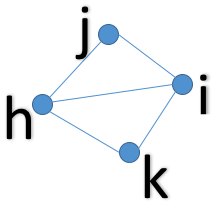
\includegraphics[width=.3\textwidth]{edge_patch2}
  		\end{center}
  		\caption{The edge patch $\langle h,i;j,k \rangle$.}
	\end{figure}
	
	\theoremstyle{definition}
	\begin{definition}{\textsc{Emersion}}
		An \emph{emersion} is a relaxation of an embedding that allows crossings. (ie. An emersion is not necessarily planar.)
	\end{definition}
	
	We will also need the notion of a \emph{dual emersion}. However, in our notion of the dual emersion, we will place $\{\infty\}$ in the center of the emersion.
	
	\begin{theorem}{(Whitney's Theorem)}
		If $G$ is a simple 3-connected, planar graph then the faces of the embedding $\pi(G)$ are uniquely defined independent of $\pi$.
	\end{theorem}
	
	As a result of Whitney's theorem, we can assign combinatorial properties to the faces of a simple 3-connected, planar graph. 
	This yields the following combinatorial structure:
	\theoremstyle{definition}
	\begin{definition}{\textsc{Combinatorial Oriented Polyhedron}}
		A \emph{combinatorial oriented polyhedron} is a finite set of vertices, faces and edge patches such that \cite{mccProof}:
		\begin{enumerate}
			\item There are two edge patches per edge. I.e. if $\langle h,i;j,k \rangle \in E$ then $\langle i,h;k,j \rangle \in E$ but $ \langle h,i;k,j \rangle \not\in E$ and $\langle h,i;j,k \rangle \not\in E$.
			\item For each vertex $a_0$ all edge patches with first entry $a_0$ form a cycle. 
			\item For each face $F^0$ all edge patches with last entry $F^0$ form a cycle.
			\item Each pair $a_0$, $a_1$ is joined by a vertex edge path. Each pair of faces is connected by a face-edge path (the vertex edge path in the dual). 
		\end{enumerate}
	\end{definition}

	\theoremstyle{definition}
	\begin{definition}{\textsc{Jordan Curve}}
		A Jordan curve or a simple closed curve in the plane $\R^2$ is the image $C$ of an one-to-one continuous map of a circle into the plane, $\phi : \mathbb{S}^1 \rightarrow \R^2$. 
	\end{definition}
	
	\begin{theorem}{(Jordan-Curve Theorem)}
		Let $C$ be a Jordan curve in the plane $\R^2$. 
		Then its complement, $\R^2 \setminus C$, consists of exactly two connected components. 
		One of these components is bounded (the interior) and the other is unbounded (the exterior), and the curve $C$ is the boundary of each component.
	\end{theorem}

	Any closed path of faces and distinct edges in a 3-connected, planar straight line graph divides the graph into two components.
	This path is a Jordan curve and therefore, by the Jordan-Curve theorem we know that both of the components will be connected. 
	From the definition of connected, we know that each of the components must have at least one vertex.
	Therefore, every closed path of faces and distinct edges will disconnect the vertices in this graph.
	
	We define this as a combinatorial object:
	
	\theoremstyle{definition}
	\begin{definition}{\textsc{Spherical Combinatorial Polyhedron}}
		A combinatorial polyhedron and its dual are spherical if every closed path of faces and distinct edges $\langle h_r,i_r;j_r,k_r \rangle$ for $1 \leq r \leq t$ such that $j_{r+1} = k_r$ and $j_1 = k_t$ disconnects the vertices \cite{mccProof}.
	\end{definition}
		
	Lastly, three other definitions that will be references are as follows:
	A \emph{cut} is a partition of the vertices of a graph into two disjoints subsets. 
	\emph{Concentric circles} are circles which share a common center and an \emph{annulus} is the space between two concentric circles with different radii \cite{mathworld:ConcentricCircles}.
	
\subsection{Proof of Maxwell-Cremona Theorem}
	We now have sufficient vocabulary to state the Maxwell-Cremona Theorem in its full technical definition.
	
	\begin{theorem}{(Maxwell-Cremona Theorem)} 
	Given an embedding with an associated spherical combinatorial polyhedron $(V,F;E)$ the following are equivalent:
		\begin{enumerate}
			\item There is a equilibrium stress on the embedding with all $\omega_e \neq 0$.
			\item There is a dual emersion on the dual graph $(F;E)$.
			\item There is a spatial polyhedron $((V,F;E);Q)$ with the embedding as its vertical projection (and the dual emersion as its face diagram).
 		\end{enumerate}
	\end{theorem}
	
	The following is a reproduction of the proof by Carpo and Whiteley \cite{mccProof}.
	
\subsubsection{Part 1: Stress and Reciprocal Diagram}
	%\theoremstyle{definition}
	%\begin{definition}{Reciprocal Framework}
		%A reciprocal framework, or dual embedding, $H* = ((F,E);P)$ on the dual combinatorial polyhedron is a framework such that for each edge patch $\langle h,i;j,k \rangle$  the vector $v_e = p_i - p_h$ is perpendicular to the vector $v^e = p^k - p^j$ from the reciprocal. 
	%\end{definition}
	
	\begin{theorem}
		A planar vertex 2-connected, edge 3-connected, straight line graph supports an equilibrium stress if and only if it has a dual emersion.
	\end{theorem}
	
	A note on notation: $90^o$ clockwise rotation will be written $u^\bot$ and $90^o$ counter-clockwise rotation will be written $-u^\bot$
	
	\begin{proof}
		Starting with a planar drawing of a graph, form the associated spherical polyhedron.
		
		Part A: Assume the spherical polyhedron has a dual emersion.
		For each edge patch $\langle h,i;j,k \rangle$ we will use the equation $\omega_{hi}(p_i - p_h) = -(P^k - P^j)^\bot$ or $\omega_ev_e = (V^e)^\bot$ to define scalars $\omega_{hi} = \omega_e$. 
		None of the weights will equal zero because $P^j \neq P^k$ in an emersion. 
		From the facial polyhedrons of the dual emersion we get $\sum\omega_ev_e = 0 = \sum\omega_{hi}(p_i - p_h)$.

		Part B: Assume we have an equilibrium stress on the embedding.
		Pick a face $F^0$ and a point $P^0$ for the this face. 
		Any other face is connected to this face by a simple face-edge path of edge patches $\{...e...\}$. 
		We define point $P^1 = P^0 + \sum\omega_ev_e^\bot$. 
		This is a consistent definition provided that two different paths from $F^0$ to $F^1$ give the same point $P^1$. 
		Two such paths form a closed path on the spherical polyhedron and therefore the edges of the path form a cut set for the graph of the polyhedron. 
		If we travel on one path and back on the other we see the sums on the two paths are equal, as required $\sum\omega_ev_e = \sum\omega_e^{'}v_e^{'} = 0$. 
		For each edge $e = \langle i,h;j,k \rangle$ the path from $P^j$ to $P^k$ is this single edge and the difference in position is $P^j - P^k = -\omega_ev_e^\bot$. 
		Thus, we have a true dual emersion.

		Part B of this proof in layman's terms is that from the definition of an equilibrium stress, a simple cycle that sums around a vertex will equal zero. 
		As a result of this fact, you can divide the graph into cut sets that each have a self stress of zero. 
		Adding these self stresses up, you obtain the final result of zero.
	\end{proof}
	
	These results generalize to any combinatorial oriented polyhedron.
	
	\begin{corollary} 
		Given a combinatorial oriented polyhedron $(V,F,E)$ and any emersion $H = ((V,E);P)$ there is an equilibrium stress on the embedding satisfying $\sum \omega_ev_e = 0$ if and only if there is a dual emersion $H* = ((F,E);P)$. 
	\end{corollary}

	\begin{proof} 
		Part A: Given a dual emersion there is an equilibrium stress.
		For any face-edge cycle $\omega_e v_e = (V^e)^{\bot}$ since the vectors $V^e$ form a closed polygon in the dual $\sum_e(V^e)^\bot = 0$.

		Part B: Given an equilibrium stress $P^1 = P^0 + \sum_e \omega_ev_e^\bot = \text{dual emersion}$.
		Given any two paths between $F^0$ and $F^1$ we get the same value for $P^1$ since the sum up one path and back the other is a cycle and yields zero.
	\end{proof}
	
	We have thus proven the first half of the Maxwell-Cremona Theorem.

	\emph{stress} $\leftrightarrow$ \emph{dual emersion}

\subsubsection{Part 2: Lifting and Reciprocal Diagrams}

	To prove the second half of the Theorem, we must first establish a few more definitions.
	
	\theoremstyle{definition}
	\begin{definition}{\textsc{Vertex Diagram}}
		The \emph{vertex diagram} of an oriented polyhedral surface $((V,F;E);Q)$ is the embedding on the projection with the graph $(V,E)$ and points $p_i = (x_i,y_i,0)$ if $q_i = (x_i,y_i,z_i)$.
	\end{definition}
	
	\theoremstyle{definition}
	\begin{definition}{\textsc{Face Diagram}}
		The \emph{face diagram} of an oriented polyhedral surface $((V,F;E);Q)$ is the emersion of the graph $(F,E)$ and points $P^i = (A^i,B^i,0)$ for $F^i$ if $Q^i = (A^i,B^i,1,C^i)$. 
		The points in the face diagram are the intersections of the plane $z=0$ with the normals to the faces through the point $(0,0,-1)$. 
		Equivalently, they are the negatives of the gradients of the face planes threaded as functions of $x$ and $y$.
	\end{definition}
	
	\theoremstyle{definition}
 	\begin{definition}{\textsc{Maxwell Polarity}}
 		The \emph{Maxwell polarity} in the space is the pair of transformations $L$ and $L^{-1}$ between points in $R^3$, triples $(x,y,z)$, and non-vertical planes in $R^3$, quadruples $(A,B,1,C)$, defined by $L(x,y,z)=(x,y,1,z)$ and $L^{-1}(A,B,1,C) = (A,B,C)$.
 	\end{definition}
	
	\begin{lemma}
		The Maxwell polarity preserves incidences: it takes a point $q$ on plane $Q$ to the plane $L(q)$ through the point if and only if the point lies on the Maxwell paraboloid $x^2 + y^2 + 2z = 0$.
 	\end{lemma}
	
	\begin{proof}
		Assume we have a point $q$ on a plane $Q$: $Ax + By + z + C = 0$. 
		After transformation to $L(q)$ and $L^{-1}(Q)$ we have: $xA + yB + C + z = 0$, so the new plane contains the new point. 
		If $q$ lies on $L(q)$ we have $x^2 + y^2 + z + z = 0$, and the point lies on the paraboloid. 
 
 		For an edge patch $e = \langle h,i;j,k \rangle$ the turning moment is $m_e = p_j \times p_i$. 
		In a similar manner, for the dual edge in the reciprocal $V^e = (P^k - P^j)$ and $M^e = P^k \times P^j = (P^k - P^j)\times P^j)$.
	\end{proof}
 
	\begin{theorem}
		Part A: For any polyhedral surface $((V,F;E);p)$ the vertex diagram and the face diagram are dual emersions.
		
 		Part B: The dependencies induced by this pair satisfy 
		(1), the vector condition $\sum \omega_e v_e = 0$ and the moment condition $\sum \omega_e m_e = 0$ and 
		(2), the dual conditions $\sum \omega^e V^e = 0$ and $\sum \omega^e M^e = 0$.
	\end{theorem}
 
 	\begin{proof}
		Part A: 
		For each face $F^i$ the vector $N^j = (A^j, B^j,1)$ is normal to the plane $Q^j$. 
		For each edge $e = \langle h,i;j,k \rangle:  (x_h-x_i,,y_h-y_i, z_h-z_i)=(q_h-q_i) = \omega^e N^j \times N^k = \omega^e(B^j-B^k,A^k-A^j,A^jB^k-A^kB^j)$. 
		This shows that $-\omega^e(A^j-A^k,B^j-B^k)^\bot = (x_h - x_i, y_h-y_i)$ or $-\omega^e(V^e)^\bot = v_e$. 
		The emersions are dual, with scalars $\omega^e$ for the equilibrium stress in the face diagram.
 
 		Part B: 
		Around any vertex-edge cycle of the polyhedron, $\sum(x_h - x_i, y_h-y_i, z_h-z_i) = 0$ and for any edge $(x_h-x_i,y_h-y_i) = -\omega^e(A^j-A^k,B^j-B^k)^\bot = -\omega^e(V^e)^\bot$. 
		Therefore, for any vertex-edge cycle in the original polyhedron, $\sum_e \omega^eV^e = \sum_e \omega^e(x_h-x_i,y_h-y_i)^\bot = 0$. 
		In addition $(z_h-z_i) = \omega^e(A^jB^k-A^kB^j) = -\omega^e(P^j-P^k) \times P^j = \omega^eM^e$. 
		Therefore, for any vertex-edge cycle in the original polyhedron $\sum \omega^eM^e = \sum(z_h-z_i) = 0$. 
 	\end{proof}
	
 	We still must show that $\sum \omega_e v_e = 0$ and that $\sum \omega_em_e = 0$ for any face-edge cycle in the vertex diagram. 

	We apply the Maxwell polarity to make the vertex diagram of the original polyhedral surface into the face diagram of the polar polyhedral surface. 
	As a face diagram it must satisfy $\sum \omega_e v_e = 0$ and $\sum \omega_em_e = 0$.

	\begin{theorem} 
		Given a dual pair of emersions $H=((V;E);p)$ and $H^* = ((F;E);P)$ on the oriented combinatorial polyhedron $(V,F;E)$ the following are equivalent: 
 		\begin{enumerate} 
 			\item The dual dependence in the original emersion satisfies $\sum \omega_em_e = 0$.
 			\item There is a polyhedral surface $((V,F;E);Q)$ with $H$ as its vertical projection and $H^*$ as its face diagram.
			\item There is a polar polyhedral surface $((F,V;E);Q^*)$ with $H^*$ as its vertical projection and $H$ as its face diagram.
			\item The dependence in the dual emersion satisfies the equation: $\sum \omega^eM^e = 0$
		\end{enumerate}
	\end{theorem}
	
	\begin{proof}
		We know that (ii) $\Rightarrow$ (iv) by the previous theorem. 

		(iv) $\Rightarrow$ (ii): 
		Choose a vertex $p_0$ and set $q_0 = (x_0, y_0,0)$. 
		For each face $P^j$ we define $N^j = (A^j,B^j,1)$, which will become its normal. 
		We recall that $\omega^eN^j \times N^k = \omega^e(B^j-B^k,A^k-A^j, A^jB^k-A^kB^j) = (V^e) + (0,0,M^e)$. 
		For every other point $p_1$ there is a vertex-edge path from $v_0$ to $v_1$. 
		We use this path to set: 
		$q_1 = q_0 + (\sum \omega^eN^j \times N^k) = (x_0,y_0,0) + (\sum \omega^eV^e + (0,0,\omega^eM^e)) = (x_0,y_0,0) + \sum \omega^eV^e + \sum \omega^eM^e = (x_1,y_1,0) + (0,0,\sum \omega_eM^e)$. 
		Since $\sum{e}\omega^eM^e = 0$ on any vertex-edge cycle, $z_1$ is well defined.

		(ii) $\Leftrightarrow$ (iii). 
		This equivalence follows from an application of the Maxwell polarity to the given polyhedral surfaces.

		(ii) $\Leftrightarrow$ (i). 
		This is the dual of (ii) $\Leftrightarrow$ (iii), and follows by the same argument. 
	\end{proof}
 
\subsubsection{Result}

	\begin{theorem}{Maxwell-Cremona Theorem}
		Given an embedding with an associated combinatorial spherical polyhedron $(V,F;E)$ the following are equivalent:
			\begin{enumerate}
				\item There is an equilibrium stress on the embedding with all $\omega_e \neq 0$.
				\item There is a dual emersion on the dual graph $(F;E)$.
				\item There is a spatial polyhedron $((V,F;E);Q)$ with the embedding as its vertical projection (and the dual emersion as its face diagram).
 			\end{enumerate}
 	\end{theorem}
	
	This result combined with Tutte's theorem can almost be used to prove \textbf{Steinitz's Theorem} which says that every planar 3-connected graph can be represented by a convex 3-dimensional polytope \cite{realizationSpaces}. 
	However this is not a complete proof because Tutte's algorithm only yields a global equilibrium stress when the outer face is a triangle. 
	Thus we have proved that every planar 3-connected graph with a triangular outer face can be represented by a convex 3-dimensional polytope. 
	Despite this limitation on the shape of the outer face, it is not difficult to prove the rest of the theorem. 
	To prove the rest of the theorem, it must be proven that if the outer face is not a triangle, then the dual will have a triangular outer face. 
	Once this has been proven, we can perform our operations on the dual and obtain Steinitz's result. 
	This is left for the reader to explore.
 
 	In total this means that every Circle packing can be represented by a Delaunay Triangulation (embedding with an equilibrium stress), which has multiple equivalent representations including, a convex 3-dimensional polytope (lifting) and a dual embedding or Voronoi Diagram. 

	This also yields intuition for a Circle packing algorithm which, though has not been proven to always work, seems to work very well on small problem instances. 
	This force-directed algorithm computes the embedding of the graph using Tutte's algorithm to iteratively modify the force of each edge by changing the distance between the two points while updating the radii of each circle iteratively. 
	The algorithm is as follows: 
	While the embedding is not a valid Circle Packing, for every edge, reposition the two vertices it connects, provided they are interior vertices, based on the stress of the edge. 
	Then, for every edge, calculate the length of the edge and determine if the radii of the two circles add up to that distance. 
	If not, increase the stress and the radii, otherwise, decrease the stress and the radii. 
	This algorithm can be observed working in our visualization tool.
 
\section{Stereographic Mappings}

	There are many equivalent representations of Circle Packings in two dimensions, namely, Weighted Delaunay Triangulations, dual circle packings, and Voronoi diagrams. 
	Additionally, from the Maxwell-Cremona theorem Circle packings can be represented as convex 3-dimensional polytopes, essentially they can be lifted into three dimensional space. 
	However, this is not the only way to represent a Circle packing in three dimensions. 
	Using Stereographic Mappings, an additional representation, on the Riemann sphere, can be discovered. 
	In this section, we will cover circle packings on the sphere and the insights this representation yields.

\subsection{Riemann Sphere}
	The Euclidean plane which has been operated on thus far can be represented mathematically by: $\C = \{z = x + iy : x, y \in \R \}$. 
	In contrast, the Riemann sphere, also known as the unit sphere or the complex projective line is modeled as such: $\mathbb{P} = \{(x,y,z):x^2 + y^2 + z^2 = 1\} \subset \R^3$. 
	This sphere can be thought of as the wrapping of the complex plane around a ball, with the addition of one point at infinity. 
	The plane is found to be a subset of the sphere via stereographic projection, which is a mapping that projects a sphere onto the plane. 
	This mapping is bijective and is often used to describe the mapping of the plane to the sphere as well. 
	Formally, start at the infinity point and draw a line towards a point on the plane. 
	This line will pass through both the sphere and the plane. 
	Let the point where the line punctures the sphere be $p = (x,y,z)$ and the point where it touches the plane point $w = u + iv$. 
	Then using similarity of triangles and recalling that $x^2 + y^2 + z^2 = 1$ the following relationships can be obtained: $u = \frac{x}{1 + z}$, $v = \frac{y}{1+ z}$. $z = \frac{1 = (u^2 + v^2}{1 + (u^2 + v^2)}$, $x = u(1+z)$, and $y =v(1+z)$.

	Circle packings can be mapped onto this sphere via stereographic projection to obtain an essentially unique circle packing. 
	This is a result of the Koebe-Andreev-Thurston Theorem which says the following \cite{stephenson05introduction}:

	\begin{theorem}{(Koebe-Andreev-Thurston Theorem)}
		Let $K$ be a combinatorial sphere. 
		Then there exists an essentially unique univalent circle packing $P_K$ for $K$ on the Riemann sphere $\mathbb{P}$.
	\end{theorem}
	
	These packings are unique up to M\"{o}bius Transformations.

	\begin{figure}[h]%
    		\centering
    		\subfloat[User input]{{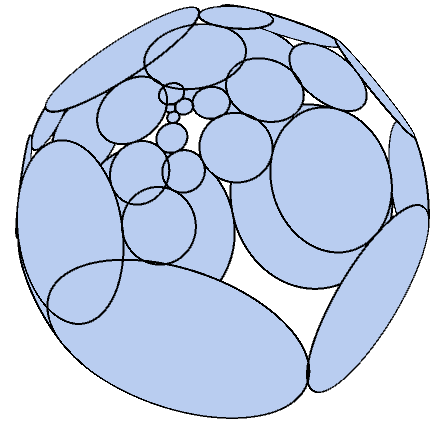
\includegraphics[width=.4\textwidth]{riemannsphere} }}%
    		\qquad
    		\subfloat[User input packed]{{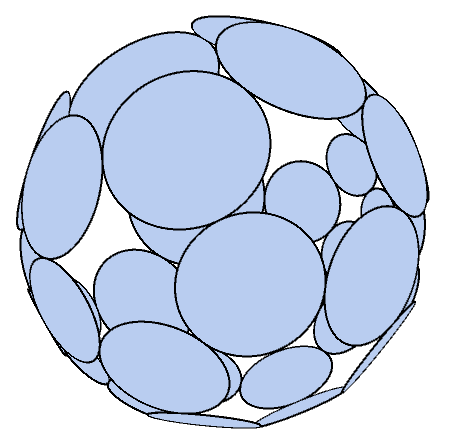
\includegraphics[width=.4\textwidth]{riemannsphere_packed} }}%
    		\caption{Stereographic projection onto the Riemann Sphere}%
    		\label{fig:riemann}%
	\end{figure}

\subsection{M\"{o}bius Transformations}
	
	A \emph{M\"{o}bius Transformation} of a plane can be obtained by performing the stereographic projection of the plane onto a sphere, then rotating or moving the sphere and then performing the stereographic projection back onto the plane. 
	
 	\theoremstyle{definition}
	\begin{definition}{\textsc{M\"{o}bius Transformation}}
		Formally, a M\"{o}bius Transformation is a rational function defined on the Riemann sphere of the form:
  		\begin{equation} 
  			f(z) = \frac{az+b}{cz+d}
  		\end{equation}
  	where $z\in\C$ is a complex variable and $a,b,c,d\in\C$ are complex numbers such that $ad - bc$ $\neq$ $0$ \cite{stephenson05introduction}. 
	\end{definition}
	
	These transformations are invertible and, if performed on circle packings, transform circle packings to equivalent circle packings without any information loss. 
	Therefore, circle packings in the plane are unique up to M\"{o}bius Transformations. 
   
    \begin{figure}[h]%
		\centering
		\subfloat[A circle packing.]{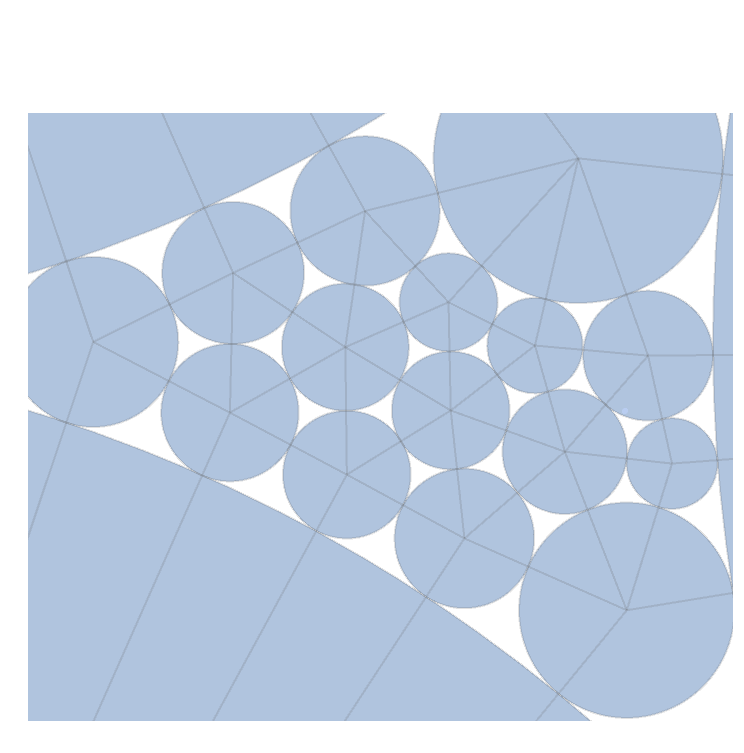
\includegraphics[width=.35\textwidth]{input_packedcropped}}%
		\qquad
		\subfloat[A M\"{o}bius Transformation of the packing in (a).]{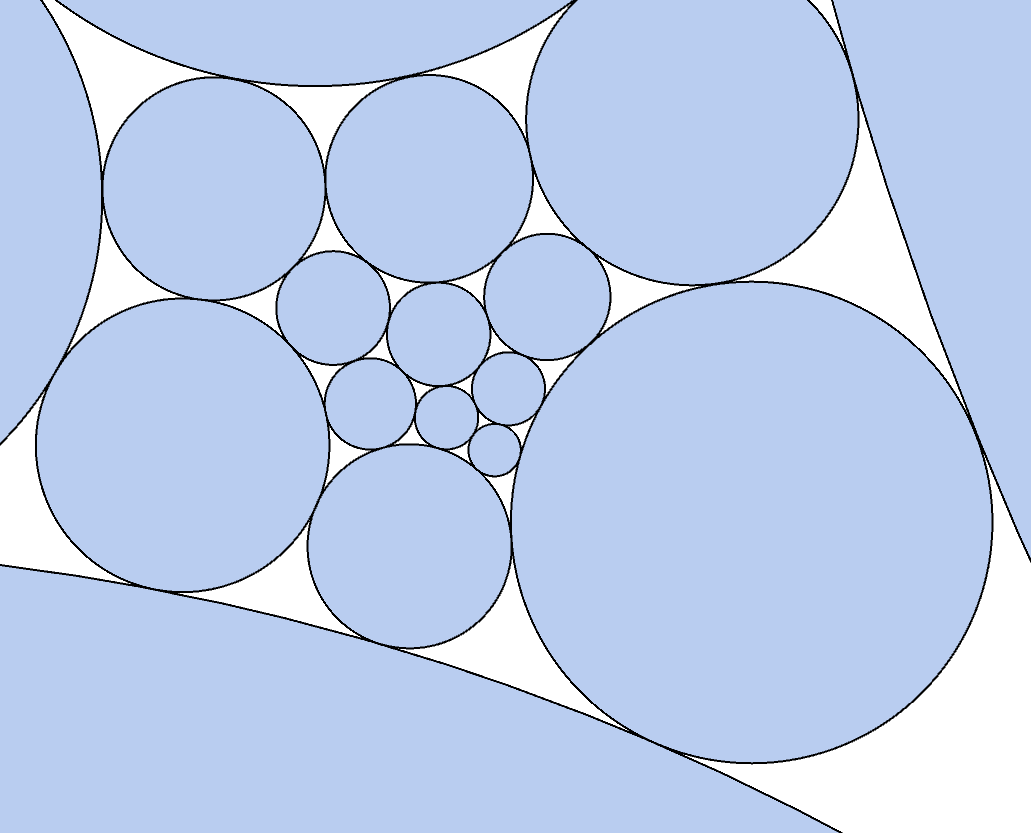
\includegraphics[width=.35\textwidth]{packing_transformed}}%
		\caption{M\"{o}bius Transformations in the plane.}%
		\label{fig:mobiusplane}%
	\end{figure}

	\begin{figure}[H]%
		\centering
		\subfloat[A Circle Packing on the sphere.]{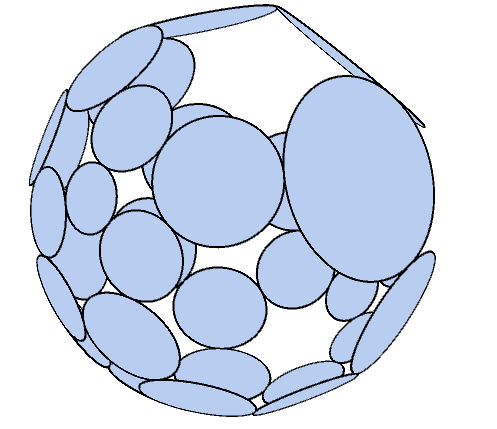
\includegraphics[width=.35\textwidth]{sphere1}}%
		\qquad
		\subfloat[A M\"{o}bius Transformation of the packing in (a).]{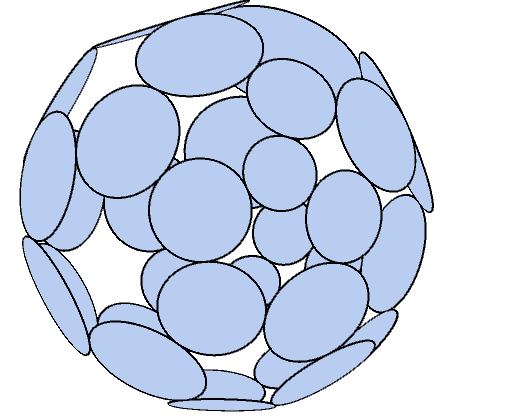
\includegraphics[width=.35\textwidth]{sphere2}}%
		\caption[]{M\"{o}bius Transformations on the Riemann Sphere.}%
		\label{fig:mobiussphere}%
	\end{figure}

\section{Conclusion}

	Circle Packings have many equivalent representations that can be exploited to develop new algorithms to both make better packings and obtain them more quickly. 
	These representations include Delaunay Triangulations, Voronoi Diagrams, Parabolic Liftings, Koebe Polyhedrons, and Packings on the Riemann Sphere. 
	Through examining one of these representations, the Delaunay Triangulation, a new algorithm for computing Circle Packings based on equilibrium forces was developed. 
	In the future, a combination of these representations could be used to develop a new non-linear optimization algorithm based on optimizing different aspects of each equivalent representation.

\section{Acknowledgements}
	I would like to thank my co-author Kevin Pratt for creating the visualization tool used to create the majority of figures for this paper. 
	Kevin is intelligent, inquisitive and knowledgable --- any readers who have questions regarding circle packings should direct them to him.
	I would also like to thank my other co-author and advisor, Don Sheehy, without whom, this paper would not be possible.
	I cannot thank Don enough for his continued support and encouragement.
	Don's guidance helped me become both a better reader and writer and without his help the quality of this paper would be nowhere near that of its current form. 
	I appreciate all the time Don spent teaching me both the basics of Computational Geometry and more specific circle packing concepts. 	
	Lastly, I would like to thank my family for all of their continued support throughout my academic career.







\bibliographystyle{plain}
\bibliography{references}
\end{document}  